\chapter{Généralités sur le courrier}
\label{chap:generalites_courrier}

\section{Introduction}
\label{sec:introduction_generalites_courrier}

Le courrier, qu’il soit traditionnel ou électronique, reste un moyen important pour échanger des informations entre les personnes, les entreprises et les administrations. Avec l’évolution des technologies numériques, le courrier électronique a pris une place très large dans les échanges quotidiens. Il permet d’envoyer rapidement des messages, des documents et des informations sans avoir besoin d’un support papier. Malgré cette facilité, son utilisation demande une bonne organisation, car les messages reçus et envoyés peuvent vite devenir nombreux et difficiles à gérer. C’est pour cette raison que la gestion du courrier électronique est devenue nécessaire pour assurer un meilleur suivi, une bonne conservation et une communication plus claire.

\begin{figure}[H]
    \centering
    % Image à chercher : évolution du courrier papier vers le courrier électronique
    % Exemple : lettre papier, ordinateur, symbole e-mail, Internet
    %\includegraphics[width=0.75\textwidth]{images/evolution_courrier.png}
    \caption{Évolution du courrier traditionnel vers le courrier électronique}
    \label{fig:evolution_courrier}
\end{figure}

\section{Définition du courrier}
\label{sec:definition_courrier}

Le courrier électronique, appelé aussi \textit{courriel}, est un moyen de communication numérique qui permet d’échanger des informations à travers un système de messagerie. Il peut être utilisé entre particuliers, dans les entreprises ou dans les administrations. Il sert à transmettre un message, mais aussi des fichiers joints, comme des documents, des images ou des formulaires \cite{bissonnette2012}.

D’un point de vue organisationnel, un courriel ne se limite pas seulement au texte envoyé. Il comprend aussi les pièces jointes et les métadonnées, comme l’expéditeur, le destinataire, l’objet, la date et l’heure d’envoi \cite{piaf}. Ces éléments sont importants, car ils permettent de mieux comprendre le contexte du message et de le conserver correctement.



\section{Défis de la gestion du courrier}
\label{sec:defis_gestion_courrier}

Dans une entreprise, la gestion des courriels n’est pas toujours simple. Avec le grand nombre de messages envoyés chaque jour, il devient parfois difficile de retrouver rapidement une information ou de bien organiser les échanges. Certains utilisateurs gardent tous leurs courriels sans les classer, ce qui surcharge les boîtes de messagerie et complique le travail au fil du temps \cite{piafgestion}.

Des problèmes de confidentialité peuvent aussi apparaître. Un message électronique peut être transféré ou copié en quelques secondes, parfois à des personnes qui ne sont pas directement concernées. Il arrive également que des documents importants soient supprimés par erreur, alors que d’autres restent stockés inutilement pendant plusieurs années \cite{piafgestion}.

Les difficultés ne concernent pas uniquement l’organisation des messages. Les outils de messagerie utilisés dans la plupart des organisations ne sont pas conçus spécialement pour l’archivage des documents. Selon Natalie Bissonnette, certains formats de sauvegarde comme HTML ou PST ne garantissent pas toujours une bonne conservation des informations liées au courriel, notamment les métadonnées \cite{bissonnette2012}. Pour cette raison, plusieurs organismes préfèrent utiliser le format PDF/A afin de conserver les courriels dans de meilleures conditions \cite{bissonnette2012}.

La manière de gérer les courriels change aussi d’une personne à une autre. Certains utilisateurs classent correctement leurs messages, alors que d’autres utilisent simplement leur boîte de réception pour conserver tous leurs documents. Cette différence dans les pratiques peut provoquer des pertes d’informations et rendre le repérage des fichiers plus compliqué \cite{piafgestion}.

\begin{figure}[H]
    \centering
    % Image à chercher : boîte mail surchargée ou gestion difficile des courriels
    % Contenu souhaité : plusieurs e-mails, notifications, surcharge, dossiers non classés
    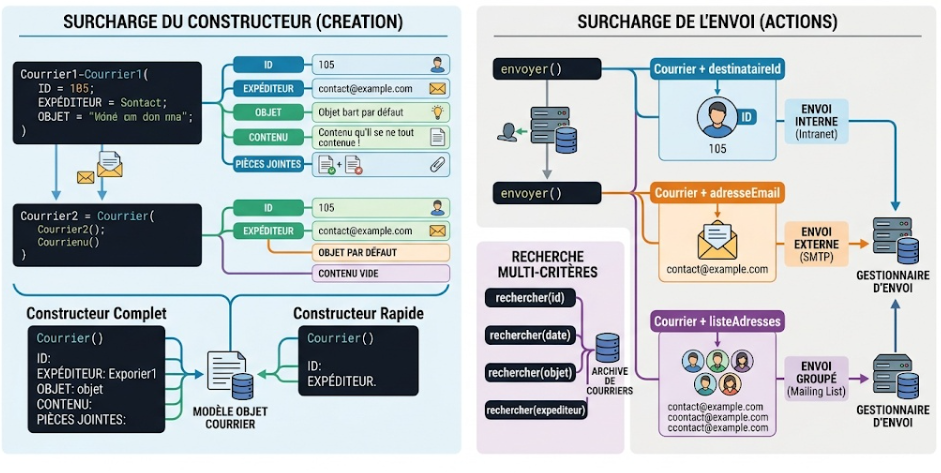
\includegraphics[width=0.75\textwidth]{images/courrier/deff.png}
    \caption{Exemple de surcharge dans la gestion des courriels}
    \label{fig:defis_gestion_courrier}
\end{figure}

\section{Importance du courrier électronique}
\label{sec:importance_courrier}

Le courrier électronique occupe une place importante dans le fonctionnement des entreprises et des administrations. Il permet d’échanger rapidement des informations, d’envoyer des documents et de garder une trace écrite des communications. Grâce à cette rapidité, plusieurs tâches peuvent être réalisées sans déplacement ni attente prolongée \cite{bissonnette2012}.

Dans le cadre professionnel, le courriel sert souvent à transmettre des décisions, des demandes, des contrats ou encore des informations liées au suivi des activités. Certains messages peuvent même avoir une valeur juridique ou administrative lorsqu’ils prouvent qu’une action a été effectuée ou qu’une décision a été prise \cite{bissonnette2012}. Pour cette raison, les organisations doivent accorder une attention particulière à leur conservation et à leur classement.

Le courrier électronique facilite aussi le travail collaboratif. Plusieurs personnes peuvent recevoir le même message, partager des fichiers ou suivre l’évolution d’un projet en temps réel. Selon Techno-Science, ce moyen de communication est apprécié pour sa rapidité, son faible coût et la possibilité d’envoyer différents types de documents numériques \cite{technoscience}.

Cependant, l’importance du courriel ne se limite pas seulement à la communication. Il joue également un rôle dans la mémoire de l’organisation. Certains échanges permettent de retracer des décisions, de comprendre le contexte d’un projet ou de conserver des informations utiles sur une longue période \cite{bissonnette2012}. C’est pour cette raison que plusieurs organismes mettent en place des politiques de gestion et d’archivage des courriels afin d’éviter les pertes d’informations et d’assurer une meilleure organisation documentaire.

\begin{figure}[H]
    \centering
    % Image à chercher : communication professionnelle par e-mail
    % Contenu souhaité : employés, ordinateur, échange de documents,
    % collaboration, messagerie professionnelle
    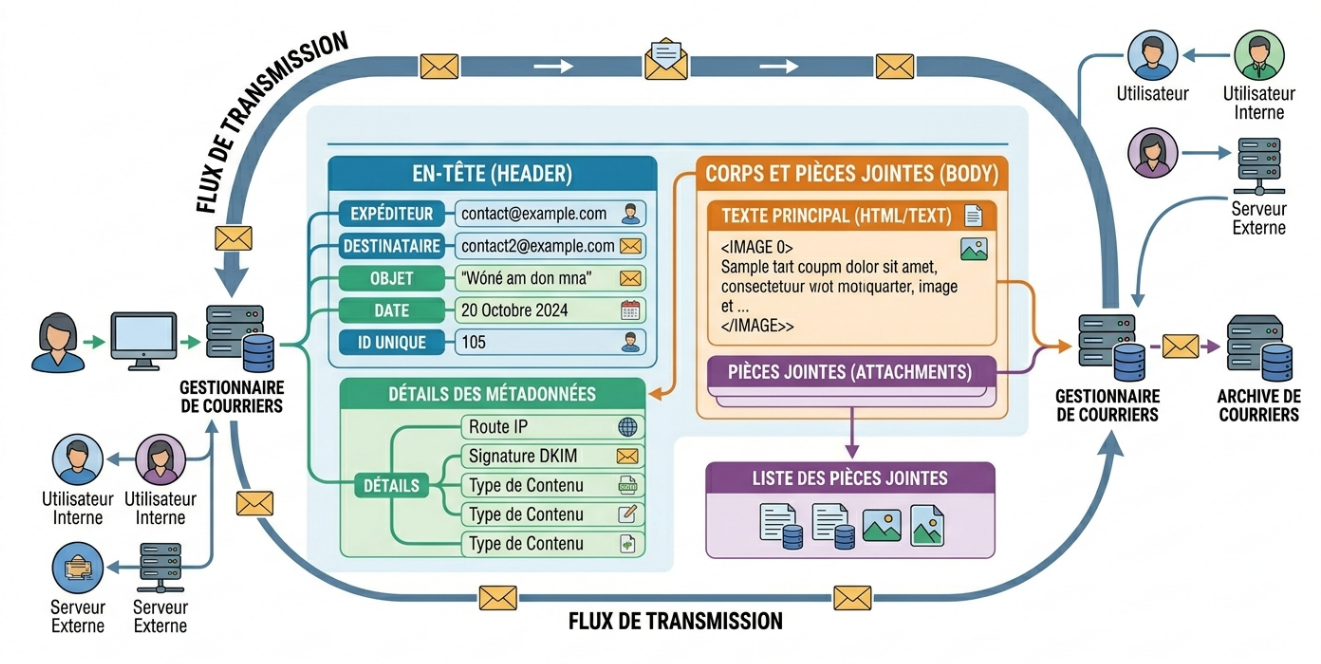
\includegraphics[width=0.75\textwidth]{images/courrier/image.png}
    \caption{Le courrier électronique dans la communication professionnelle}
    \label{fig:importance_courriel}
\end{figure}


\section{Conclusion}
\label{sec:conclusion_generalites_courrier}

Dans ce chapitre, nous avons présenté les notions générales liées au courrier électronique ainsi que son rôle dans les échanges professionnels et administratifs. Le courriel facilite la communication et le partage rapide des informations, ce qui explique son utilisation dans presque toutes les organisations.

Nous avons aussi vu que la gestion des courriels ne se limite pas seulement à l’envoi et à la réception des messages. Elle concerne également le classement, la conservation et la sécurité des informations échangées. Plusieurs difficultés peuvent apparaître, surtout lorsque les messages sont nombreux ou mal organisés.

Enfin, les applications de gestion de courrier permettent d’améliorer le suivi des échanges et de réduire les risques de perte d’informations. Le chapitre suivant sera consacré à l’étude et à la conception de notre application de gestion de courrier électronique.
